\documentclass[journal]{vgtc}\usepackage[]{graphicx}\usepackage[]{color}
%% maxwidth is the original width if it is less than linewidth
%% otherwise use linewidth (to make sure the graphics do not exceed the margin)
\makeatletter
\def\maxwidth{ %
  \ifdim\Gin@nat@width>\linewidth
    \linewidth
  \else
    \Gin@nat@width
  \fi
}
\makeatother

\definecolor{fgcolor}{rgb}{0, 0, 0}
\newcommand{\hlnum}[1]{\textcolor[rgb]{0,0,0}{#1}}%
\newcommand{\hlstr}[1]{\textcolor[rgb]{0.502,0,0}{#1}}%
\newcommand{\hlcom}[1]{\textcolor[rgb]{0,0,0}{#1}}%
\newcommand{\hlopt}[1]{\textcolor[rgb]{0,0,0}{#1}}%
\newcommand{\hlstd}[1]{\textcolor[rgb]{0,0,0}{#1}}%
\newcommand{\hlkwa}[1]{\textcolor[rgb]{0,0,1}{#1}}%
\newcommand{\hlkwb}[1]{\textcolor[rgb]{0,0,0}{#1}}%
\newcommand{\hlkwc}[1]{\textcolor[rgb]{0,0,1}{#1}}%
\newcommand{\hlkwd}[1]{\textcolor[rgb]{0,0,0}{#1}}%

\usepackage{framed}
\makeatletter
\newenvironment{kframe}{%
 \def\at@end@of@kframe{}%
 \ifinner\ifhmode%
  \def\at@end@of@kframe{\end{minipage}}%
  \begin{minipage}{\columnwidth}%
 \fi\fi%
 \def\FrameCommand##1{\hskip\@totalleftmargin \hskip-\fboxsep
 \colorbox{shadecolor}{##1}\hskip-\fboxsep
     % There is no \\@totalrightmargin, so:
     \hskip-\linewidth \hskip-\@totalleftmargin \hskip\columnwidth}%
 \MakeFramed {\advance\hsize-\width
   \@totalleftmargin\z@ \linewidth\hsize
   \@setminipage}}%
 {\par\unskip\endMakeFramed%
 \at@end@of@kframe}
\makeatother

\definecolor{shadecolor}{rgb}{.97, .97, .97}
\definecolor{messagecolor}{rgb}{0, 0, 0}
\definecolor{warningcolor}{rgb}{1, 0, 1}
\definecolor{errorcolor}{rgb}{1, 0, 0}
\newenvironment{knitrout}{}{} % an empty environment to be redefined in TeX

\usepackage{alltt}                % final (journal style)
%\documentclass[review,journal]{vgtc}         % review (journal style)
%\documentclass[widereview]{vgtc}             % wide-spaced review
%\documentclass[preprint,journal]{vgtc}       % preprint (journal style)
%\documentclass[electronic,journal]{vgtc}     % electronic version, journal

%% Uncomment one of the lines above depending on where your paper is
%% in the conference process. ``review'' and ``widereview'' are for review
%% submission, ``preprint'' is for pre-publication, and the final version
%% doesn't use a specific qualifier. Further, ``electronic'' includes
%% hyperreferences for more convenient online viewing.

%% Please use one of the ``review'' options in combination with the
%% assigned online id (see below) ONLY if your paper uses a double blind
%% review process. Some conferences, like IEEE Vis and InfoVis, have NOT
%% in the past.

%% Please note that the use of figures other than the optional teaser is not permitted on the first page
%% of the journal version.  Figures should begin on the second page and be
%% in CMYK or Grey scale format, otherwise, colour shifting may occur
%% during the printing process.  Papers submitted with figures other than the optional teaser on the
%% first page will be refused.

%% These three lines bring in essential packages: ``mathptmx'' for Type 1
%% typefaces, ``graphicx'' for inclusion of EPS figures. and ``times''
%% for proper handling of the times font family.

\usepackage{mathptmx}
\usepackage{graphicx}
\usepackage{times}
\usepackage{amsmath}
\usepackage{stmaryrd}%\rightarrowtriangle
\usepackage{graphicx}
\usepackage{enumerate}
\usepackage{natbib}
\usepackage{url}

%% We encourage the use of mathptmx for consistent usage of times font
%% throughout the proceedings. However, if you encounter conflicts
%% with other math-related packages, you may want to disable it.

%% This turns references into clickable hyperlinks.
\usepackage[bookmarks,backref=true,linkcolor=black]{hyperref} %,colorlinks
\hypersetup{
  pdfauthor = {},
  pdftitle = {},
  pdfsubject = {},
  pdfkeywords = {},
  colorlinks=true,
  linkcolor= black,
  citecolor= black,
  pageanchor=true,
  urlcolor = black,
  plainpages = false,
  linktocpage
}

% Reduce space between enumerations
\newenvironment{tight_enumerate}{
\begin{enumerate}
  \setlength{\itemsep}{0pt}
  \setlength{\parskip}{0pt}
}{\end{enumerate}}

%% If you are submitting a paper to a conference for review with a double
%% blind reviewing process, please replace the value ``0'' below with your
%% OnlineID. Otherwise, you may safely leave it at ``0''.
\onlineid{0}

%% declare the category of your paper, only shown in review mode
\vgtccategory{Research}

%% allow for this line if you want the electronic option to work properly
\vgtcinsertpkg

%% In preprint mode you may define your own headline.
%\preprinttext{To appear in IEEE Transactions on Visualization and Computer Graphics.}

%% Paper title.
\title{Extending ggplot2's grammar of graphics implementation for linked and dynamic graphics on the web}

%% This is how authors are specified in the journal style

%% indicate IEEE Member or Student Member in form indicated below
\author{Carson Sievert, Toby Dylan Hocking, Susan VanderPlas, Jun Cai, Kevin Ferris}
\authorfooter{
\item
 Toby Dylan Hocking is with the McGill University department of Human Genetics. E-mail: toby.hocking@mail.mcgill.ca
\item
 Carson Sievert is with the Department of Statistics at Iowa State University. E-mail: sievert@iastate.edu
\item
 Susan VanderPlas is with the Department of Statistics at Iowa State University. E-mail: srvanderplas@gmail.com
\item
  Jun Cai is with the Center for Earth System Science at Tsinghua University. E-mail: cai-j12@mails.tsinghua.edu.cn
\item
  Kevin Ferris is with the Department of Statistics at Montana State University. E-mail: kevin.ferris10@gmail.com
}

%other entries to be set up for journal
\shortauthortitle{Biv \MakeLowercase{\textit{et al.}}: Global Illumination for Fun and Profit}
%\shortauthortitle{Firstauthor \MakeLowercase{\textit{et al.}}: Paper Title}

%% Abstract section.
\abstract{ 
  The web is the most popular medium for sharing interactive
  data visualizations thanks to the portability of the web browser and
  the accessibility of the internet. Unfortunately, creating
  interactive web graphics often requires a working knowledge of
  numerous web technologies that are foreign to many people working
  with data. As a result, web graphics are rarely used for exploratory
  data analysis where quick iteration between different visualizations
  is of utmost importance. This is the core strength of ggplot2, a
  popular data visualization package for the world's leading
  open-source statistical programming language, R. The conceptual
  framework behind ggplot2 is based on the grammar of graphics, which
  lays a foundation for describing any static graphic as a small set
  of independent components. Perhaps the most fundamental component is
  the mapping from abstract data to the visual space, sometimes
  referred to as the aesthetic mapping. We propose adding two new
  aesthetics to the grammar, which together are sufficient for
  elegantly describing both animations and certain classes of
  coordinated linked views. We implement this extension in the
  open-source R package animint, which converts ggplot2 objects to
  interactive web visualizations via D3.  
} % end of abstract

%% Keywords that describe your work. Will show as 'Index Terms' in journal
%% please capitalize first letter and insert punctuation after last keyword
\keywords{Interactive graphics, Statistical graphics, Exploratory data analysis, Web technologies}

%% Uncomment below to include a teaser figure.
%    \teaser{
%    \centering
%    \includegraphics[width=16cm]{CypressView}
%    \caption{In the Clouds: Vancouver from Cypress Mountain.}
%   }

%% Uncomment below to disable the manuscript note
%\renewcommand{\manuscriptnotetxt}{}

%% Copyright space is enabled by default as required by guidelines.
%% It is disabled by the 'review' option or via the following command:
% \nocopyrightspace

%%%%%%%%%%%%%%%%%%%%%%%%%%%%%%%%%%%%%%%%%%%%%%%%%%%%%%%%%%%%%%%%
%%%%%%%%%%%%%%%%%%%%%% START OF THE PAPER %%%%%%%%%%%%%%%%%%%%%%
%%%%%%%%%%%%%%%%%%%%%%%%%%%%%%%%%%%%%%%%%%%%%%%%%%%%%%%%%%%%%%%%%
\IfFileExists{upquote.sty}{\usepackage{upquote}}{}
\begin{document}

%% The ``\maketitle'' command must be the first command after the
%% ``\begin{document}'' command. It prepares and prints the title block.

%% the only exception to this rule is the \firstsection command
\firstsection{Introduction}

\maketitle

%% In general, there are three influential roles involving an Animint
%% visualization: the developer, who implements the Animint library; the
%% designer, who uses the Animint library to define a visualization; and
%% the user, who selects data subsets to view in a web browser. The main
%% goal of Animint is to provide an expressive language for designers,
%% while allowing users the freedom to interact with the plot to
%% selectively view data subsets of interest. The designer specifies data
%% sets and maps variables to interactive visual elements using the
%% Animint DSL, then uses the Animint library to compile and save an
%% interactive animation. The user writes no code, but can view and
%% interact with an Animint visualization by clicking Scalable Vector
%% Graphics (SVG) elements in a web browser. The Animint library
%% developer is responsible for the plot rendering details, which allows
%% the others to focus on designing and consuming visualizations.



%%Interactive and dynamic statistical graphics toolkits play an important role in the exploratory phase of a data analysis cycle. The web is an attractive platform for interactive graphics thanks to its portability and accessibility, but due to a lack of tools for quick iteration, web graphics are not a practical tool for exploring data. Instead, they are mostly used for the presentation of findings (i.e., when the 'correct' visualization is already known). This is a source of conflict, as one often needs different tools depending on whether the work is exploratory or intended for public consumption, which results in wasted effort.

%%The R package \texttt{ggplot2} is a popular tool for data visualization due in part to its elegant design inspired by the grammar of graphics. The fundamental concept in the grammar of graphics is that any graphic can be described through a set of mappings from data variables to visual space, referred to commonly as \texttt{aesthetic} mappings. The grammar of graphics and ggplot2 were designed for static graphics


The world's leading open source statistical programming language, R, has a rich history of interfacing with computational tools for the use of people doing data analysis and statistics research \citep{RCore}. Understanding R's core audience is important, as they typically want to maximize their time working on data analysis problems, and minimize time spent learning computational tools. R excels in this regard, as it is designed specifically for interactive use, where users can quickly explore their data using highly expressive interfaces. Another key player in R's success story is its packaging infrastructure, which provides tools for distributing entire research conpendium(s) (code, data, documentation, auxiliary documents, etc) \citep{Gentleman:Lang}. 

One of the most widely used R packages is ggplot2 \citep{ggplot2-book}, a data visualization package inspired by the grammar of graphics \citep{wilkinson}. In fact, \citet{Donoho:2015tu} writes: ``This effort may have more impact on today’s practice of data analysis than many highly-regarded theoretical statistics papers".
In our experience, ggplot2 has made an impact thanks to its foundation in the grammar of graphics, carefully chosen defaults, and overall usability. This helps data analysts rapidly iterate and discover informative visualizations -- an essential task in exploratory data analysis (EDA). When dealing with high-dimensional data, however, it is often useful to produce interactive and/or dynamic graphics, which ggplot2 does not inherently support. 

%%Since the design space of interactive and dynamic graphics is so large, however, it is extremely difficult to design an fully featured interface that is useful in a EDA setting.

Interactive graphics toolkits in R have been used for decades to enhance the EDA workflow, but these approaches are often not easy to reproduce or distribute to a larger audience. It is true that most graphics generated during EDA are ultimately not useful, but sometimes, understanding gained during this phase is most easily shared via the interactive graphics themselves. Thus, there is value is being able to easily share, and embed interactive graphics inside a larger report. Unfortunately, this is typically hard, if not impossible, using traditional interactive graphics toolkits. As a result, there is a large disconnect between the visualization tools that we use for exploration versus presentation. 

We aim to narrow this gap in visualization tools by extending ggplot2's grammar of graphics implementation for interactive and dynamic web graphics. By adding two new aesthetics to the grammar, \texttt{clickSelects} and \texttt{showSelected}, we are able to express animated transitions and perform linked queries on graphical elements like those described in \citep{Ahlberg:1991} and \citep{Buja:1991vh}. Other aesthetics, such as \texttt{tooltip} and \texttt{href}, can be used to identify data values and link to web pages. The rest of the paper will proceed as follows: Section~3 discusses the \texttt{clickSelects} and \texttt{showSelected} aesthetics in detail, Section~4 discusses our current implementation in the R package animint, Section~5 compares our implementation to similar work, Section~6 provides a handful of examples, ...


\section{Related Work}

We aim to provide a system which empowers ggplot2 users to go beyond the confines of static graphics with minimal friction introduced into their current workflow. We acknowledge that numerous systems which support similar visualization techniques exist outside of the R ecosystem, but we intentionally focus on R interfaces since the statistical computing environment it provides is essential for many exploratory data analysis tasks.

In terms of the user interface, the R package gganimate is very similar to our system \citep{gganimate}. It directly extends ggplot2 by adding a new aesthetic, named \texttt{frame}, which splits the data into subsets (one for each unique value of the frame variable), produces a static plot for each subset, and uses the animation package to combine the images into a key frame animation \citep{animation}. The concept is quite similar, but not as powerful, as using the \texttt{showSelected} aesthetic and \texttt{time} option in our system. Either system has the ability to control the amount of time that a given frame is displayed, but our system can also animate the transition between frames. Smooth transitions are generally useful for tracking positions between frames, which is crucial in many scenarios, such as the touring example discussed in Section~6.

Tours are a useful visualization technique for exploring high-dimensional data which requires interactive and dynamic graphics. The open source software ggobi is currently the most fully-featured tool for touring data, but also provides the ability to produce more standard statistical graphics, and general interactive techniques such as linking, zooming, panning, and identifying \citep{ggobi:2007}. The R package rggobi \citep{rggobi} provides an R interface to ggobi's graphical interface, but unfortunately, the software requirements for installation and use of this toolchain are heavy and stringent. Furthermore, sharing the interactive versions of these graphics are not possible. The R package cranvas aims to be the successor to ggobi, with support for similar interactive techniques, but with a more flexible interface for describing plots inspired by the grammar of graphics \citep{cranvas}. Cranvas also has heavy and stringent software requirements which limits the portability and accessibility of the software.

Another R package for interactive graphics which draws design inspiration from the grammar of graphics is ggvis \citep{ggvis}. It does not directly extend ggplot2, but instead provides a brand new purely functional interface which is designed with interactive graphics in mind. It currently relies on Vega to render the SVG graphics from JSON \citep{vega}, and the R package shiny to enable many of its interactive capabilities \citep{shiny}. The interface gives tremendous power to R users, as it allows one to write R functions to handle user events. This power does come with a cost, though, as sharing and hosting ggvis graphics may require special web server software, even when the interaction logic could be handled entirely client-side. As we outline in Section~4, our system does not require a web server, but can be used inside shiny web applications, when desired.

\section{The \texttt{clickSelects} and \texttt{showSelected} keywords for interactive
  plot design}
\label{sec:design}

%% In the system we propose, the central concept of interactivity is a
%% selection variable, such as year or region in Figure~1. For each
%% selection variable, one or several values can be selected at a time,
%% e.g. year=1979 and country=\{United States, Vietnam\}.  Like
%% Cleveland's system, we also use enhanced linking to highlight the
%% selected value(s) of each selection variable. In contrast to
%% Cleveland's single rectangular brush that selects points in plots of a
%% single data table, we propose several selection variables in linked
%% plots of several data tables. Linking is accomplished using common
%% names when declaring \texttt{clickSelects} and \texttt{showSelected}
%% selection variables.

%% For example, to declare a clickable plot element that changes the
%% selected value of the year variable, a designer writes
%% \texttt{clickSelects=year} (tallrect in Figure~1). And to show only
%% the data subset for the selected value of year, a designer writes
%% \texttt{showSelected=year} (point and text in Figure~1).

%% Using just the \texttt{clickSelects} and \texttt{showSelected}
%% keywords, a wide variety of interactive visualizations can be
%% defined. To make the selection automatically change over time
%% (animation), a designer may declare one variable as the \texttt{time}
%% variable. Since it is perceptually advantageous to have smooth
%% transitions in data-driven animations \citep{animated-transitions}, a
%% designer may also declare a \texttt{duration} list of selection
%% variables which should have smooth transitions.

In this section we explain the meaning of the new
\texttt{clickSelects} and \texttt{showSelected} keywords that we
propose to use for interactive graphic design. We
propose using these keywords as new aesthetics in the ggplot2 system
\citep{ggplot2-book}. An aesthetic is a declarative mapping from a
data variable to a property of a geometric plot element. Some standard
ggplot2 aesthetics are
\begin{description}
\item[x] horizontal position,
\item[y] vertical position,
\item[color] color or fill,
\item[size] point or line thickness.
\end{description}
We propose adding two new aesthetics to define interactions:
\begin{description}
\item[clickSelects] clicking changes the current selection,
\item[showSelected] show only data for the current selection.
\end{description}

We use a visualization based on the World Bank data set to explain
the usage of these new aesthetics. The World Bank data consist of
several economic variables measured for 205 countries from 1960 to
2012 \citep{WorldBank}. Figure~1 shows a visualization consisting of
two linked plots based on these data. In the static PDF version of
this figure, the year 1979 and the countries United States and Vietnam
are selected, but readers are encouraged to interactively select other
values using a web
browser.\footnote{\url{http://bl.ocks.org/tdhock/raw/8ce47eebb3039263878f/}}
In the interactive version, the selected value of the year variable is
automatically incremented every few seconds, using animation to
visualize yearly changes in the relationship between life expectancy
and fertility rate.

\begin{figure*}[b!]
  \centering
  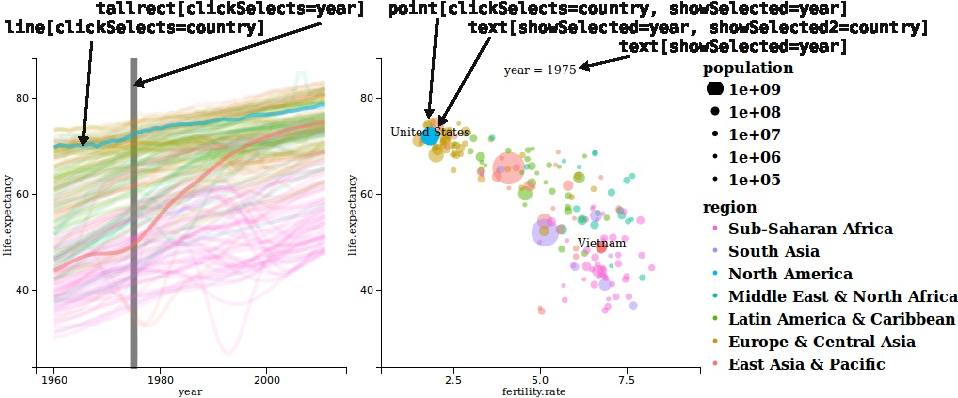
\includegraphics[width=\textwidth]{figure-1}
  \caption{An interactive animation of World Bank demographic data of
    several countries, designed using \texttt{clickSelects} and
    \texttt{showSelected} keywords (top).  \textbf{Left}: a multiple
    time series from 1960 to 2010 of life expectancy, with bold lines
    showing the selected countries and a vertical grey tallrect
    showing the selected year. \textbf{Right}: a scatterplot of life
    expectancy versus fertility rate of all countries. The legend and
    text elements show the current selection: year=1979,
    country=$\{\textrm{United States}, \textrm{Vietnam}\}$, and
    region=$\{\textrm{East Asia \& Pacific}, \textrm{North
      America}\}$}
  \label{fig:1}
\end{figure*}

The World Bank data visualization consists of five geometric elements,
each with different interactive aesthetics (top of Figure~1). The time
series on the left of Figure~1 contains two geometric elements:
tallrect and line. We define the tallrects in the background based on
the \texttt{years} data set, which has one row for every year between
1960 and 2010:

\begin{knitrout}
\definecolor{shadecolor}{rgb}{1, 1, 1}\color{fgcolor}\begin{kframe}
\begin{alltt}
\hlstd{yearRects} \hlkwb{<-} \hlkwd{geom_tallrect}\hlstd{(}
  \hlkwd{aes}\hlstd{(}\hlkwc{xmin}\hlstd{=year}\hlopt{-}\hlnum{0.5}\hlstd{,} \hlkwc{xmax}\hlstd{=year}\hlopt{+}\hlnum{0.5}\hlstd{,}
      \hlkwc{clickSelects}\hlstd{=year),}
  \hlkwc{data}\hlstd{=years)}
\end{alltt}
\end{kframe}
\end{knitrout}

The tallrect plots a rectangle that spans the entire vertical range,
for each row of the \texttt{years} data set. The horizontal range of
each rectangle is specified by the \texttt{xmin} and \texttt{xmax}
aesthetics. The \texttt{clickSelects=year} aesthetic means that
clicking on a tallrect should change the selected year. For example,
if the rectangle for 1980 is clicked, the selected year should change
to 1980.
%% Finally,
%% \texttt{alpha=1/2} specifies that the selected tallrect should have an
%% opacity of 50\%. Since color is black by default, this results in a
%% selected semi-transparent tallrect which appears grey. Since
%% non-selected \texttt{clickSelects} plot elements have 1/2 less opacity
%% by default, this results in non-selected rectangles which are
%% completely transparent, blending in with the white background.


%% Animint also provides a shorthand syntax for tallrects, as they are a
%% common geom/aesthetic pairing in linked plots.

%% <<yearRects-make>>=
%% yearRects <- make_tallrect(WorldBank, "year")
%% @

%% This approach allows us to utilize both plots to display meaningful
%% information: we can overlay the tallrects in the first plot with time
%% series data while still using the tallrects to modify the second
%% plot. Similar linked graphs could be produced with D3, but the grammar
%% of graphics approach allows for fewer lines of code and simpler
%% debugging.

To create the time series plot, we create a ggplot that combines the
tallrects above with lines based on the entire World Bank data set:

\begin{knitrout}
\definecolor{shadecolor}{rgb}{1, 1, 1}\color{fgcolor}\begin{kframe}
\begin{alltt}
\hlstd{timeSeries} \hlkwb{<-} \hlkwd{ggplot}\hlstd{()}\hlopt{+}
  \hlstd{yearRects}\hlopt{+}
  \hlkwd{geom_line}\hlstd{(}
    \hlkwd{aes}\hlstd{(}\hlkwc{x}\hlstd{=year,} \hlkwc{y}\hlstd{=life.expectancy,}
        \hlkwc{group}\hlstd{=country,} \hlkwc{color}\hlstd{=region,}
        \hlkwc{clickSelects}\hlstd{=country,}
        \hlkwc{showSelected}\hlstd{=region),}
    \hlkwc{data}\hlstd{=WorldBank)}
\end{alltt}
\end{kframe}
\end{knitrout}

To define the lines we used both interactive aesthetics. The
\texttt{clickSelects=country} definition means that clicking a line
should change the selected country. The \texttt{showSelected=region}
definition means to only plot the subset of data that corresponds to
the current selection of the \texttt{region} variable.

Note that the tallrect used \texttt{data=years} whereas the line used
\texttt{data=WorldBank}. The multi-layer ggplot2 system allows a
different data set for each layer/geom. Interactivity is accomplished
by defining interactive aesthetics using common variable names in the
different data sets. For example, the \texttt{year} variable is common
to both the \texttt{WorldBank} and \texttt{years} data sets.

Having completed the definition of the time series plot on the left of
Figure~1, now let us consider the scatterplot on the right. The
following R code defines the points in the scatterplot:

\begin{knitrout}
\definecolor{shadecolor}{rgb}{1, 1, 1}\color{fgcolor}\begin{kframe}
\begin{alltt}
\hlstd{countryPoints} \hlkwb{<-} \hlkwd{geom_point}\hlstd{(}
    \hlkwd{aes}\hlstd{(}\hlkwc{x}\hlstd{=fertility.rate,} \hlkwc{y}\hlstd{=life.expectancy,}
        \hlkwc{color}\hlstd{=region,} \hlkwc{size}\hlstd{=population,}
        \hlkwc{clickSelects}\hlstd{=country,}
        \hlkwc{showSelected}\hlstd{=year,}
        \hlkwc{showSelected2}\hlstd{=region),}
    \hlkwc{data}\hlstd{=WorldBank)}
\end{alltt}
\end{kframe}
\end{knitrout}

The code creates a point for every row in the World Bank data
table. The visual characteristics of each point are defined by the
values of the corresponding data: the (x,y) position encodes fertility
rate and life expectancy, point color encodes the region, and point
size encodes the population. Note that scales are automatically
constructed for the x and y axes, and legends are automatically
constructed for color and size. The \texttt{clickSelects=country}
aesthetic means that clicking a point should change the selected
country. The \texttt{showSelected=year} and
\texttt{showSelected2=region} aesthetics mean to only plot the points
that match both the selected year and region.

In order to remind the plot user which subset of data are selected, we
will draw text labels for the selected year and countries. First, we
create the year labels using

\begin{knitrout}
\definecolor{shadecolor}{rgb}{1, 1, 1}\color{fgcolor}\begin{kframe}
\begin{alltt}
\hlstd{yearText} \hlkwb{<-} \hlkwd{geom_text}\hlstd{(}
  \hlkwd{aes}\hlstd{(}\hlkwc{label}\hlstd{=}\hlkwd{sprintf}\hlstd{(}\hlstr{"year = %d"}\hlstd{, year),}
      \hlkwc{showSelected}\hlstd{=year),}
  \hlkwc{x}\hlstd{=}\hlnum{5}\hlstd{,} \hlkwc{y}\hlstd{=}\hlnum{80}\hlstd{,}
  \hlkwc{data}\hlstd{=years)}
\end{alltt}
\end{kframe}
\end{knitrout}

The \texttt{label} aesthetic is used to define the text from the year
variable, and only the selected year is shown due to the
\texttt{showSelected=year} aesthetic. Note that since the label
\texttt{x} and \texttt{y} positions are constant, they are not defined
as aesthetics.

We can also add another label to show the selected countries:

\begin{knitrout}
\definecolor{shadecolor}{rgb}{1, 1, 1}\color{fgcolor}\begin{kframe}
\begin{alltt}
\hlstd{countryText} \hlkwb{<-} \hlkwd{geom_text}\hlstd{(}
    \hlkwd{aes}\hlstd{(}\hlkwc{x}\hlstd{=fertility.rate,} \hlkwc{y}\hlstd{=life.expectancy,}
        \hlkwc{label}\hlstd{=country,}
        \hlkwc{showSelected}\hlstd{=country,}
        \hlkwc{showSelected2}\hlstd{=year,}
        \hlkwc{showSelected3}\hlstd{=region),}
    \hlkwc{data}\hlstd{=WorldBank)}
\end{alltt}
\end{kframe}
\end{knitrout}

A geom/layer may contain any number of \mbox{showSelected}
aesthetics. In this example, the three \texttt{showSelected}
aesthetics mean to only show the subset of labels corresponding to the
selected country, year, and region.

Having defined these three geometric elements, we combine them in a
single ggplot:

\begin{knitrout}
\definecolor{shadecolor}{rgb}{1, 1, 1}\color{fgcolor}\begin{kframe}
\begin{alltt}
\hlstd{scatterPlot} \hlkwb{<-} \hlkwd{ggplot}\hlstd{()}\hlopt{+}
  \hlstd{countryPoints}\hlopt{+}
  \hlstd{yearText}\hlopt{+}
  \hlstd{countryText}
\end{alltt}
\end{kframe}
\end{knitrout}

This completes the definition of the scatterplot. Note that both the
\texttt{timeSeries} and \texttt{scatterPlot} objects are valid
ggplots, even though they use the new \texttt{clickSelects} and
\texttt{showSelected} aesthetics. However, plotting these objects
using ggplot2 will render non-interactive plots with all geometric
elements, including data for all years and countries. In the next
section, we propose the \texttt{animint} R package, which implements a new
interactive renderer for ggplots with the \texttt{clickSelects} and
\texttt{showSelected} aesthetics.

%% \begin{figure*}[b!]
%%   \centering
%%   \begin{tabular}{ccc}
%%   \begin{minipage}{2.5in}
%%     \centering
%%     \textbf{D3 (Javascript code)}
%%     \small
%% \begin{verbatim}
%% svg.selectAll("circle")
%%   .data(one_year)
%%   .enter().append("circle")
%% .attr("cx", function(d){
%%   return x_scale(d.fertility_rate);
%% }).attr("cy", function(d){
%%   return y_scale(d.life_expectancy);
%% }).attr("r", function(d){
%%   return size_scale(d.population);
%% }.style("fill", function(d){
%%   return color_scale(d.region);
%% })
%% \end{verbatim}
%%   \end{minipage}
%%   &
%%   \begin{minipage}{2.6in}
%%     \centering
%%     \textbf{Vega (JSON file)}
%%     \small
%% \begin{verbatim}
%% { "marks": [{
%%   "type":"symbol",
%%   "from": {"data":"this_year"},
%%   "properties":{ "enter":{
%%     "x": {"field": "fertility_rate"},
%%     "y": {"field": "life_expectancy"},
%%     "size": {"field": "population"},
%%     "fill": {"field": "region"}
%% }}}]}
%% \end{verbatim}
%%   \end{minipage}
%%   &
%%   \begin{minipage}{2in}
%%     \centering
%%     \textbf{Animint (R code)}
%%     \small
%% \begin{verbatim}
%% geom_point(aes(
%%   x=fertility.rate,
%%   y=life.expectancy,
%%   color=region,
%%   size=population,
%% \end{verbatim}
%%     {\color{red}
%% \begin{verbatim}
%%   clickSelects=country,
%%   showSelected=year),
%% \end{verbatim}
%%       }
%% \begin{verbatim}
%%   data=WorldBank)
%% \end{verbatim}
%%     \end{minipage}
%%   \end{tabular}
%%   \caption{Comparison of code used to define points on a scatterplot.
%%     Note that the Animint code is shorter and simpler than the D3 and
%%     Vega code. Animint and Vega provide nice defaults for plot elements such
%%     as the axes and labels, but these elements still need to be expressed
%%     in the D3 code. Also, Animint implements the proposed
%%     \texttt{clickSelects} and \texttt{showSelected} aesthetics (red),
%%     but D3 and Vega do not.}
%%   \label{fig:code}
%% \end{figure*}

%% Carson: This seems like an opportunity to compare to Vega.
%% Animint is similar in the respect that the renderer takes
%% a JSON object as it's 'input', but it doesn't have the equivalent
%% of Animint's compiler.

\section{Current implementation in the \texttt{animint} R package}

Since 2013 we have been developing the \texttt{animint} R
package,\footnote{freely available at
  \url{https://github.com/tdhock/animint}} which provides an
interactive renderer for ggplots with \texttt{clickSelects} and
\texttt{showSelected} aesthetics. We first explain how a graphic
designer can use \texttt{animint} to render a set of ggplots, then explain the
graphical user interface (GUI) for selecting data subsets. Finally, we
discuss some implementation details of the compiler and renderer,
which only the \texttt{animint} package developers need to be concerned about.

\subsection{Animint renderer for a list of ggplots}

We will again use the World Bank data visualization of Figure~1 as an
example. Recall that in Section~3 we defined two ggplot objects,
\texttt{scatterPlot} and \texttt{timeSeries}. To plot them with
\texttt{animint}, we first put them in a named list:

\begin{knitrout}
\definecolor{shadecolor}{rgb}{1, 1, 1}\color{fgcolor}\begin{kframe}
\begin{alltt}
\hlstd{viz} \hlkwb{<-}
  \hlkwd{list}\hlstd{(}\hlkwc{scatterPlot}\hlstd{=scatterPlot,}
       \hlkwc{timeSeries}\hlstd{=timeSeries,}
       \hlkwc{time}\hlstd{=}\hlkwd{list}\hlstd{(}\hlkwc{variable}\hlstd{=}\hlstr{"year"}\hlstd{,} \hlkwc{ms}\hlstd{=}\hlnum{3000}\hlstd{),}
       \hlkwc{duration}\hlstd{=}\hlkwd{list}\hlstd{(}\hlkwc{year}\hlstd{=}\hlnum{1000}\hlstd{),}
       \hlkwc{selector.types}\hlstd{=}\hlkwd{list}\hlstd{(}
         \hlkwc{year}\hlstd{=}\hlstr{"single"}\hlstd{,}
         \hlkwc{country}\hlstd{=}\hlstr{"multiple"}\hlstd{,}
         \hlkwc{region}\hlstd{=}\hlstr{"multiple"}\hlstd{))}
\end{alltt}
\end{kframe}
\end{knitrout}

The \texttt{viz} list contains two ggplots and three options:
\texttt{time}, \texttt{duration}, and \texttt{selector.types}. The
\texttt{time} option specifies that in absence of user interaction, we
want the plots to animate over time, progressing at a rate of one year
every 3 seconds (ms = milliseconds). The \texttt{duration} option
specifies that when updating the selected year, there should be a
smooth transition with a duration of 1 second. Smooth transitions are
useful to emphasize continuity between plotted objects before and after the
transition \citep{animated-transitions}. Finally, the
\texttt{selector.types} option is used to define either single or
multiple selection for each variable. For single selection, only one
value is selected at any time (e.g. year=1990). For multiple
selection, a set of values is selected (e.g. country=$\{\textrm{United
  States}, \textrm{Vietnam}\}$).

The \texttt{viz} list contains all of the information that we need to
create the linked plots of Figure~1. To render the plots, we call the
\texttt{animint2dir} function:

\begin{knitrout}
\definecolor{shadecolor}{rgb}{1, 1, 1}\color{fgcolor}\begin{kframe}
\begin{alltt}
\hlkwd{animint2dir}\hlstd{(viz,} \hlkwc{out.dir}\hlstd{=}\hlstr{"figure-WorldBank"}\hlstd{)}
\end{alltt}
\end{kframe}
\end{knitrout}

The \texttt{animint2dir} function saves some data files and a web page
in the \texttt{figure-WorldBank} directory, then it opens the
interactive plot in a web browser.

\subsection{User interaction}

In this section we explain how a user can view and interact with a
data visualization produced by the \texttt{animint} system. As explained in the
previous section, the \texttt{animint} system outputs a set of data files along
with a web page. Opening the web page in a web browser will render the
data visualization and allow the user to select different subsets of data
to plot.

When viewing an \texttt{animint} data visualization in a web browser,
interactions are accomplished mainly via direct
manipulation. \citet{instrumental-interaction} discussed the
advantages of direct manipulation in graphical user
interfaces. \texttt{Animint} data visualizations are inspired by principle 2,
``Physical actions on objects vs. complex syntax.'' In particular, the
user can update the selection by directly clicking on the geoms with
\texttt{clickSelects} aesthetics. Also, \texttt{animint} creates a multiple
selection variable for each discrete legend (e.g. region in
Figure~1). Clicking on an entry in a discrete legend will update the
corresponding selection variable. This use of direct manipulation
contrasts other systems which use menus and widgets, and thus suffer
from less articulatory directness \citep{Hutchins:1985}.

For single selection variables such as year, clicking sets the value
of the corresponding selection variable. For multiple selection
variables such as country, clicking adds or removes values from the
set of selected values.

While it is often best to interact by directly clicking on the plotted
data, there are situations where indirect manipulation is
preferable. For example, when there are many different values that
could be selected, it is convenient to have a menu that contains all
possible values. More concretely, suppose that we would like to add
Thailand to the selected set of countries in Figure~1. The
\texttt{animint} renderer provides a selection menu which shows the
full list of countries, and allows entering text to search for a
particular country (Figure~\ref{fig:widgets}).


\begin{figure}[b!]
  \centering
  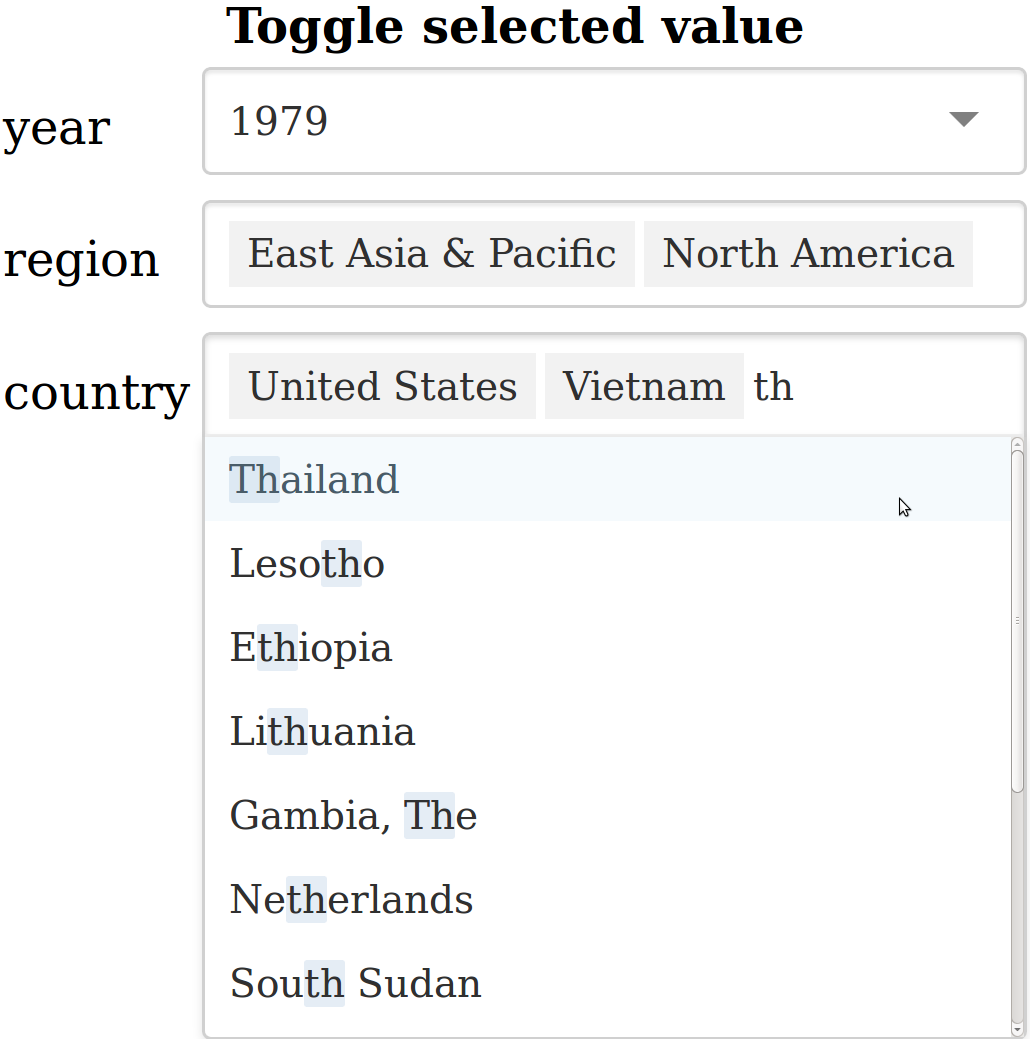
\includegraphics[width=0.5\columnwidth]{Screenshot-toggle-selected-value}
  \caption{Animint provides a menu to update each selection
    variable. In this example, after typing ``th'' the country menu
    shows the subset of matching countries.}
  \label{fig:widgets}
\end{figure}

\subsection{Implementation details}
\label{sec:implementation}

As shown in Figure~\ref{fig:design}, the \texttt{animint} system is implemented
in 2 parts: the compiler and the renderer.

\begin{figure}[b!]
  \centering
  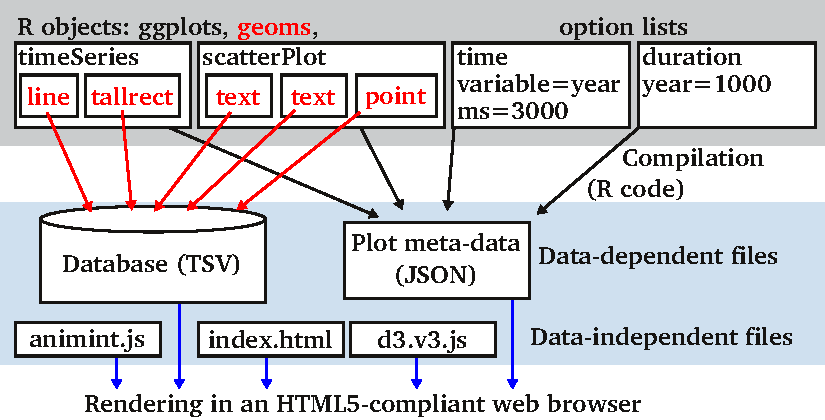
\includegraphics[width=\columnwidth]{figure-design}
  \caption{Schematic explanation of compilation and rendering the
    World Bank visualization shown in Figure~1. \textbf{Top}: the
    interactive animation is a list of 4 R objects: 2 ggplots and 2
    option lists. \textbf{Center}: \texttt{animint} R code compiles data in
    ggplot geoms to a database of TSV files
    (\textcolor{red}{$\rightarrowtriangle$}). It also compiles plot
    meta-data including ggplot aesthetics, animation time
    options, and transition duration options to a JSON meta-data file
    ($\rightarrowtriangle$). \textbf{Bottom}: those data-dependent
    compiled files are combined with data-independent JavaScript and
    HTML files which render the interactive animation in a web browser
    (\textcolor{blue}{$\rightarrowtriangle$}).}
  \label{fig:design}
\end{figure}

\begin{figure*}[p]
  \centering
  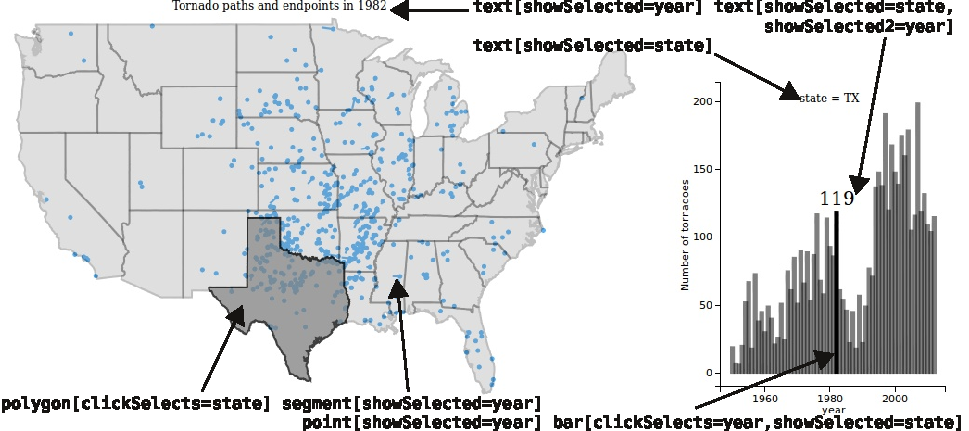
\includegraphics[width=\textwidth]{figure-tornado}
  \caption{Interactive animation of tornadoes recorded from 1950 to
    2012 in the United States. \textbf{Left}:
    map of the lower 48 United States with tornado paths in 1982. The
    text shows the selected year, and clicking the map changes the
    selected state, currently Texas. \textbf{Right}: time series of
    tornado counts in Texas. Clicking a bar changes the selected year,
    and the text shows selected state and the number of tornadoes
    recorded there in that year (119 tornadoes in Texas in 1982).}
  \label{fig:tornado}
\end{figure*}

\begin{figure*}[p]
  \centering
  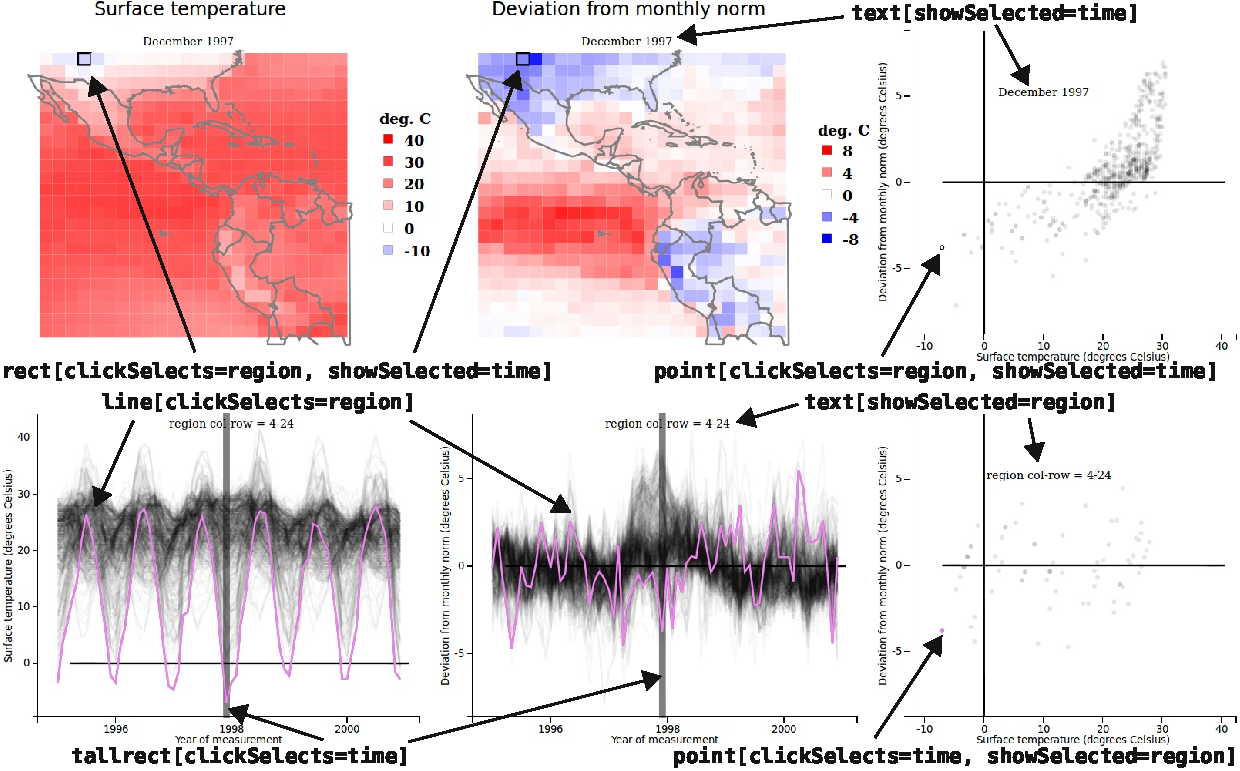
\includegraphics[width=\textwidth]{figure-climate}
  \caption{Visualization containing 6 linked, interactive, animated
    plots of Central American climate data. \textbf{Top}: for the selected time
    (December 1997), maps displaying the spatial distribution of two
    temperature variables, and a scatterplot of these two
    variables. The selected region is displayed with a black outline,
    and can be changed by clicking a rect on the map or a point on the
    scatterplot. \textbf{Bottom}: time series of the two temperature
    variables with the selected region shown in violet, and a
    scatterplot of all times for that region. The selected time can be
   changed by clicking a background tallrect on a time series or a
    point on the scatterplot. The selected region can be changed by
    clicking a line on a time series.}
  \label{fig:climate}
\end{figure*}

\begin{figure*}[b!]
  \centering
  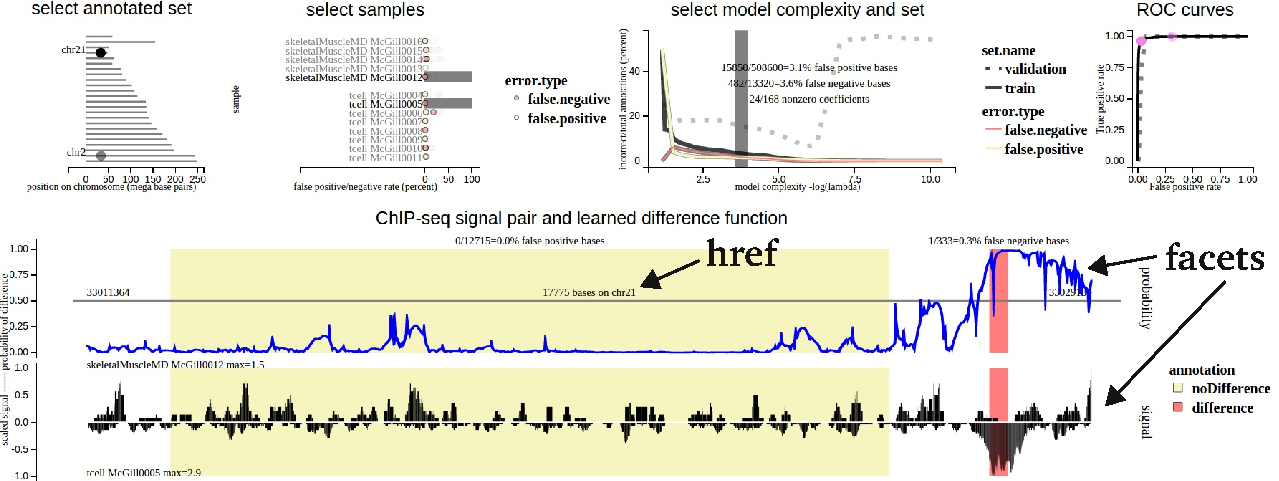
\includegraphics[width=\textwidth]{figure-chip-seq}
  \caption{Visualization with 4 selection variables used to navigate
    through 1,292,464 rows of data in 5 linked interactive plots. The
    bottom plot shows a facets plot with aligned x axes, used to
    emphasize that the blue probability function is defined at the
    same positions as the black signals below. It also contains an
    href tag (web link), which opens a new genome browser web page
    zoomed to the same region as the selected data.}
  \label{fig:ChIPseq}
\end{figure*}

The compiler is implemented in about 2000 lines of R code that
converts a list of ggplots and options to a JSON plot meta-data file
and a tab-separated values (TSV) file database
(Figure~\ref{fig:design}).

The compiler scans the aesthetics in the ggplots to determine
how many selection variables are present, and which geoms to update
after a selection variable is updated. It uses ggplot2 to
automatically calculate the axes scales, legends, labels, backgrounds,
and borders. It outputs this information to the JSON plot meta-data
file.

The compiler also uses ggplot2 to convert data variables (e.g. life
expectancy and region) to visual properties (e.g. y position and
color). The data for each layer/geom are saved in several TSV files,
one for each combination showSelected values. Thus for large data
sets, the web browser only needs to download the subset of data
required to render the current selection \citep{2013-immens}.

When repeated data would be saved in each of the TSV files, an extra
common TSV file is created so that the repeated data only need to be
stored and downloaded once. In that case, the other TSV files do not
store the common data, but are merged with the common data after
downloading. This method for constructing the TSV file database was
developed to minimize the disk usage of \texttt{animint}, particularly
for ggplots of spatial maps as in Figure~\ref{fig:tornado}.

Finally, the rendering engine (\texttt{index.html}, \texttt{d3.v3.js},
and \texttt{animint.js} files) is copied to the plot directory. The
\texttt{animint.js} renderer is implemented in about 2200 lines of
JavaScript/D3 code that renders the TSV and JSON data files as SVG in
a web browser. Importantly, animation is achieved by using the
JavaScript \texttt{setInterval} function, which updates the
\texttt{time} selection variable every few seconds. Since the compiled
plot is just a directory of files, the interactive plots can be hosted
on any web server. The interactive plots can be viewed by opening the
\texttt{index.html} page in any modern web browser.

\section{Results and comparison study on World Bank data}
\label{sec:compare}

To show the advantages that the \texttt{animint} grammar brings for creating
interactive and animated data visualizations, we implemented the World
Bank visualization of Figure~1 using two other R packages and Tableau. The main result of our comparison (Table~\ref{tab:packages}) is that
\texttt{animint} requires significantly fewer lines of code, and produces
interactive plots with more articulatory directness
\citep{Hutchins:1985}. Note that it is possible to implement the World
Bank visualization in pure D3 (Figure~\ref{fig:code}), but would
require significantly more code. % The reference of fig:code is missing.

\subsection{R package animation}
\label{sec:compare-animation}

We designed a version of the WorldBank visualization with limited
interactivity, using 38 lines of R code and the animation
package. The main idea behind this approach is to use an imperative
programming style with for loops to create a static PNG image for each
year of the data, and then show these images in sequence. The main
drawback to this approach is that the resulting plot is only
interactive with respect to the year variable. In other words, the
designer must select some countries to emphasize, and the user can not
change that selection. Another drawback is that R package
animation does not support smooth transitions between
animation frames. In contrast, using only 20 lines of the \texttt{animint} DSL,
the \texttt{animint} package achieves smooth transitions and interaction with
respect to both year and country variables.

\begin{table}[t!]
%% Table captions on top in journal version
  \caption{Implementation complexity and features
    of the World Bank data visualization
    %of Figure~1
    using several libraries that can create interactive animations.
    For each library
    we show the number of lines of code (LOC), the on-screen objects
    that can be clicked,  the
    number of interaction variables, and URL of the interactive version.
%  Note that different countries can not be interactively selected using
% the visualization created with R package animation.
% The URLs are missing.
  }
 \label{tab:packages}
% \scriptsize
 \begin{center}
  \begin{tabular}{cccccc}
    library &
    LOC &
    click on &
    %language &
    %years &
    interaction vars &
    http://bit.ly/
    \\
    \hline
    \texttt{animint} &
    20 &
    plotted data &
    %R &
    %2013- &
    several &
    \\
    \texttt{animation} &
    38 &
    play/pause &
    %R  &
    %2007- &
    1 = time &
    \\
    %% D3 &
    %% TODO &
    %% JavaScript &
    %% %2011- &
    %% several &
    %% %declarative &
    %% \\
    \texttt{ggvis}/\texttt{shiny} &
    84 &
    widgets &
    %R  &
    %2012- &
    several &
    \\
    Tableau &
      &
    widgets/plot &
    several &
    \\
  \end{tabular}
 \end{center}
\end{table}

\subsection{Client-server systems like ggvis/shiny}

We designed another version of the World Bank data visualization in 84
lines of R code (\url{http://bit.ly/1diUYsg}), using the ggvis
graphics library combined with the recommended shiny web server
package \citep{shiny, ggvis}. Showing and hiding data subsets was
accomplished by clicking on a slider for year and a menu for country,
not by clicking on the plot elements. In contrast, we designed
Figure~1 using only 20 lines of R code with the \texttt{animint} package.
Implementation is significantly simpler using \texttt{animint}
because \texttt{animint}'s DSL is designed specifically for this type of
interactive animation.
%Although creating such visualizations in ggvis+shiny is
%possible, it requires significantly more work for limited
%interactivity.

The two packages also have different features for interacting with a
data visualization: ggvis uses sliders, checkboxes, and other HTML
form elements, whereas \texttt{animint} users can directly click the SVG
elements that are used to visualize the data. For example, a ggvis of
the WorldBank data would animate over the years by adding a play/pause
button to a slider widget which controls the selected year. In
contrast, in \texttt{animint} we used a multiple time series plot where the
year can be selected by directly clicking the data values on the plot
(Figure~1). The \texttt{animint} plot is thus easier for the user since it has
more articulatory directness \citep{Hutchins:1985}, and less spatial
offset \citep{instrumental-interaction}.

Another difference is the amount of work required to deploy or share a
visualization. A compiled \texttt{animint} visualization consists of static
TSV, JSON, HTML, and JavaScript files which can be easily served with
any web server. In contrast, ggvis+shiny requires a web server with R
and special software installed, significantly complicating
deployment to the web.

There are also inherent speed tradeoffs to using a client-server
plotting system like ggvis+shiny rather than an entirely web
client/JavaScript-based system like \texttt{animint}. There is one main
difference between these two types of systems that affects
responsiveness of a web-based interactive plotting system:
client-server communication overhead. All the \texttt{animint}
JavaScript plot rendering code is executed in the web browser, whereas
ggvis executes some computations on the server. This means that after
a mouse click, ggvis can not update a plot immediately, but instead
must wait for the server to respond with the plot data.

We quantified speed differences between the two systems by timing web
page loading using DevTools in the Chromium web browser Version
33.0.1750.152, on Ubuntu 12.04 (256984). We also used \texttt{getTime()}
in JavaScript to record timings for interactive plot updates (on a
desktop computer with a 2.8GHz Intel Core i7 CPU). Using ggvis with a
local web server and the World Bank data resulted in a web page that
loaded quickly (about 1.4s), but updated the plot with a noticeable
lag after each mouse click (500--1000ms). Note that since we used a
local web server, these times represent the overhead of the web server
system, and would be larger with a remote web server.

\begin{table*}[b!] % This table is too wide to fill in the page.
  \centering
  % latex table generated in R 3.0.2 by xtable 1.7-3 package
% Fri Mar 21 10:48:45 2014
\begin{tabular}{rrrrrrrrrrr}
  \hline
 & lines of R code & seconds & MB & rows & onscreen & variables & interactive & plots & animated? & Fig \\ 
  \hline
worldPop & 17 & 0.2 & 0.1 & 924 & 624 &  4 &  2 &  2 & yes &  \\ 
  WorldBank & 20 & 2.5 & 2.3 & 34132 & 11611 &  6 &  2 &  2 & yes &  1 \\ 
  evolution & 25 & 24.7 & 12.5 & 240600 & 2703 &  5 &  2 &  2 & yes &  \\ 
  change & 36 & 3.4 & 2.7 & 36238 & 25607 & 12 &  2 &  3 & no &  \\ 
  tornado & 39 & 1.7 & 6.2 & 103691 & 16642 & 11 &  2 &  2 & no &  2 \\ 
  prior & 54 & 0.8 & 0.2 & 1960 & 142 & 12 &  3 &  4 & no &  \\ 
  breakpoints & 66 & 0.6 & 0.3 & 4242 & 667 & 13 &  2 &  3 & no &  \\ 
  compare & 66 & 12.2 & 7.8 & 133958 & 2140 & 20 &  2 &  5 & no &  \\ 
  climate & 87 & 14.6 & 21.5 & 253856 & 88980 & 15 &  2 &  6 & yes &  3 \\ 
   \hline
\end{tabular}

  \vskip 0.2cm
  \caption{Characteristics of 11 interactive visualizations designed with
    \texttt{animint}. From left to right, we show the data set name, the
    lines of R code (LOC) including data processing but not including comments
    (80 characters max per line),
    the amount of time it takes to compile the visualization (seconds),
    the total size of the uncompressed TSV files in megabytes (MB),
    the total number of data points (rows),
    the median number of data points shown at once (onscreen),
    the number of data columns visualized (variables),
    the number of \texttt{clickSelects}/\texttt{showSelected} variables (interactive),
    the number of linked panels (plots),
    if the plot is animated,
    and the corresponding Figure number in this paper (Fig).
  }
\label{tab:examples}
\end{table*}

When we used \texttt{animint} to make the World Bank data visualization, the
compilation from R objects to 2.1MB of uncompressed TSV data files
took 2.3s. Using a local web server, the \texttt{animint} JavaScript rendered
the plot very quickly (100--200ms). We also observed very fast plot
updates after mouse clicks in \texttt{animint}: 20--30ms response times for
selecting the year, and 60--70ms response times for selecting the
country.
%Furthermore, in web server systems the client may not cache
%previously viewed subsets, which results in calculations inefficiently
%being performed several times rather than simply saved for quick
%viewing later.

The conclusion of our speed comparison is that the overhead of waiting
for a web server to perform computations results in significant
slowdowns for interactive animations. It is clear that for quick
response times, it is preferable to use an entirely JavaScript-based
system like \texttt{animint}.

In contrast, a web server system like ggvis+shiny would be more
appropriate for
%  interactive animations that have many more subsets of
% the data than can ever be transferred over the network. In that case,
% the web server will initially send only the first data subset, and
% then send only the subsets of data that the client requests. However,
% since the data sets we examined were not too large
% (Table~\ref{tab:examples}), client-side rendering using Animint
% resulted in quick, responsive interactive animations.
% Another application for which a web server system like ggvis+shiny
% would be preferable is for
performing arbitrary calculations in R/C code on the server, in
response to user inputs, and then sending the result across the
network for plotting in the user's web browser. This power is not
always necessary for interactive animations, since the only operation
needed is showing precomputed data subsets. However, the web server
system would certainly be preferable when there are many more data
subsets than could ever be precomputed. In that case, the web server
would only compute the subsets that the user interactively specifies.

\subsection{Tableau}

We implemented a version of the WorldBank data visualization using
Tableau's GUI (\url{http://bit.ly/worldBank-tableau}).
%% TDH 20 Nov 2014: When I click on a country on the scatterplot it
%% does not select that country's time series --- is that an inherent
%% limitation of Tableau that we should discuss?
It was impossible to implement all features of the multiple time
series plot of the data visualization, since it includes multiple
layers with different data sources and variable mappings (a line for
each country and a tallrect for each year). Since each mark in a
Tableau plot must use the same data source, it was impossible to
control the clickable multiple time series and the clickable tallrects
in different ways based on the two different selection variables. In
conclusion, although Tableau is useful for many simple interactive
data visualizations, it is inherently limited in ways that
\texttt{animint} is not.

Tableau's GUI and visual query approach
make it easy to design several kinds of linked plots, but it does not
easily acheive the same level of flexibility that \texttt{animint}/ggplot2's
layered grammar of graphics provides. In particular, ggplot2 allows
for each layer of geoms in a plot to have a different data source and
variable mapping, while Tableau requires each mark of a plot to be a
function of a single query result. This results in a substantial
conceptual difference between the selection models of Tableau and
\texttt{animint}. In Tableau, there is a selection set for each plot, which may
include several different marks. In contrast, \texttt{animint} keeps track of a
selection set for each selection variable, each of which has
geom-specific effects based on the geom's \texttt{clickSelects}/\texttt{showSelected}
variables.


\section{Example applications}

In this section we discuss the range of examples that we have designed
with \texttt{animint}. Table~\ref{tab:examples} shows several characteristics
of 11 interactive visualizations that we have designed using
\texttt{animint}.

We quantified the implementation difficulty of the \texttt{animint} examples
using lines of R code, including data processing but not including
comments (80 characters max per line). We counted the number of plots
and variables shown to quantify the amount of information conveyed by
the visualization. Using only 17 lines of code, we designed a simple
visualization that shows 2 linked plots of 4 variables in the worldPop
data set. In contrast, the most complex visualization required 229
lines of code, and it shows 44 variables across 5 linked plots
(Figure~\ref{fig:ChIPseq}). All of the visualizations that we designed
involved at least 2 interaction variables (e.g. year and country in
Figure~1) and 2 plots. Indeed, \texttt{animint} is most appropriate for
interactive visualizations of multivariate data that are not easy to
view all at once in one plot.

Table~\ref{tab:examples} also shows \texttt{animint} system requirements for
plots of various sizes. We timed the compilation step in R code
(``seconds'' column), and measured the size in megabytes of the
compiled TSV file database (``MB'' column), and found that both
increase with the data set size (``rows'' column).
%Although we do not present timings for the rendering step,
We also noticed that the time required for the interactive updates and
rendering increases with the amount of data displayed at once
(``onscreen'' column). In particular, the climate data visualization
has noticeably slow animations, since it displays about 88,980
geometric elements at once (\url{http://bit.ly/QcUrhn}). We observed
this slowdown across all browsers, which suggested that there is an
inherent bottleneck when rendering large interactive plots in web
browsers using JavaScript and SVG. Another \texttt{animint} with a similar
amount of total rows is based on the evolution data
(\url{http://bit.ly/O0VTS4}), but since it shows less data onscreen
(about 2703 elements), it exhibits faster responses to interactivity
and animation.

\subsection{Animated examples}

Animation is very useful for data sets which have a time variable,
as in the World Bank data of Figure~1.

Figure~\ref{fig:tornado} shows an interactive animation of tornadoes
observed in the United States between 1950 and 2012. At any moment in
time, the user can simultaneously view the spatial distribution of
tornadoes in the selected year over all states, and see the trend over
all years for the selected state. Clicking a state on the map updates the
time series bars to show the tornado counts from that state. Clicking
a bar on the time series updates the selected year.

Figure~\ref{fig:climate} shows an interactive animation of climate
time series data observed in Central America. Two maps display the
spatial distribution of two temperature variables, which are shown
over time in corresponding the time series plots below. Scatterplots
also show the relationships between the two temperature variables for
the selected time and region. Clicking any of the plots updates all 6
of them. The \texttt{clickSelects} and \texttt{showSelected} aesthetics make it easy to
design this set of 6 linked plots in only 87 lines of code.
%% Animint's
%% DSL allows for this level of flexibility while using minimal lines of
%% code to define the plots and the relationship between them.

\subsection{Non-animated examples}

Animint is still useful for creating interactive but
non-animated plots when there is not a time variable in the data.
In fact, 7 of the 11 examples in
Table~\ref{tab:examples} are not animated. For example, linked plots
are useful to illustrate complex concepts such as a change point
detection model in the breakpoints data
(\url{http://bit.ly/1gGYFIV}). The user can explore different model
parameters and data sets since these are encoded as \texttt{animint}
interaction variables.

Another non-animated example is Figure~\ref{fig:ChIPseq}, which was
used to explain a complex machine learning model for predicting
differences between samples. The interactive visualization allows the
user to explore how the predictions change as a function of the model
complexity parameter, in several train and test samples. It also uses
facets, a feature from ggplot2 that allows multi-panel plots with
aligned axes. Finally, it includes hyperlinks which open related web
pages in new windows.

Overall, we have found that \texttt{animint} is useful for exploring
relationships in many different kinds of multivariate data. By using
\texttt{clickSelects} and \texttt{showSelected}, it is easy to design
interactive plots that reveal patterns in complex data.

\section{User feedback and observations}

By working with researchers in several fields of research,
we have created a wide variety of
interactive visualizations using \texttt{animint}.
Typically, the researchers have a complex data set that
they wish to visualize,
but they do not have the expertise or time to create
an interactive data visualization.
The \texttt{animint} DSL made it easy to collaborate with the various domain experts,
who were able to provide us with annotated sketches of the desired plots,
which we then translated to \texttt{animint} R code.
In this section we share comments and
constructive criticism that we have obtained from our users.

\subsection{Designer perspective}

R users have found that \texttt{animint} is easy to learn. One statistics
Ph.D. student writes, ``animint is a fantastic framework for creating
interactive graphics for someone familiar with R and ggplot2's grammar
of graphics implementation. The API is very intuitive and allows one
to quickly bring their static graphics to life in a way that
facilitates exploratory data analysis.''

TODO: expand to address reviewer comments.

\subsection{User perspective}

For the \texttt{prior} data visualization
(\url{http://bit.ly/1peIT7t}), the \texttt{animint} user is a machine learning
researcher who developed an algorithm and applied it to 4 benchmark
data sets. He wanted to explore how his algorithm performed, in
comparison to a baseline learning algorithm. He appreciated the
intuition about his algorithm's performance that he learned from the
interactive plots: ``Interactive plotting allows us to explore all
relationships of our high-dimensional dataset and gives us an
intuitive understanding of the performance of our proposed
algorithm. An intuitive understanding of the results is important
since it shows under which conditions our proposed method works well
and provides avenues for further research.''

Another user from a machine learning background found the interactive
plots useful for presenting his work: ``the `regularization path' is a
difficult concept to demonstrate in my research. The \texttt{animint}
(\url{http://bit.ly/1gVb8To}) helped greatly by rendering an
interactive plot of regularization path, likelihood, and graph at the
same time and illustrating their connections. It also reveals an
interesting phenomenon that maximizing the testing likelihood actually
gives many false positives.''

In another application, the \texttt{animint} user was a genomics researcher:
``viewing and exploring my complex intestinal microbiome dataset in
\texttt{animint} allowed me to grasp the patterns and relationships between
samples at an almost intuitive level. The interactive aspect of it was
very helpful for browsing through the dataset.''

Finally, users also appreciated the simple web interface, and the
detail that is possible to show in interactive plots, but impossible
to show in publications: ``...  the web interface is simple and easy
to use.  It also enables us to publish more detailed interactive
results on our website to accompany the results presented in
publications.''

\section{Discussion}

Finally, another key strength of ggplot2 and D3 for visualization
design are the libraries' declarative syntax, which allows a
visualization designer to specify \emph{what} they want to render
rather than \emph{how} to render it. \citet{declarative} proposed a
declarative syntax for animated transanitions, and studied the
benefits of declarative languages for data visualization. \texttt{Animint} is
another declarative DSL, but defined at a higher level of abstraction
than D3. It enables designers to focus on data visualization, while
the \texttt{animint} library developers can work on improving the lower-level
rendering details.

\subsection{Value of sketching}

The first step in the design of any data visualization is usually to
make a sketch of the desired interactive plot on paper or a
whiteboard.  In any plot a designer would sketch the axes, legends, a
few geometric elements, and note which variables will be shown in the
linked plots. An \texttt{animint} designer needs only add the
\texttt{clickSelects} and \texttt{showSelected} mappings for
each geometric element, as shown in Figures~1, 3, and 4. These notes
can be directly translated to ggplot2 aesthetics in R code, as
explained below.

% More paragraphs are needed in this subsection.

\section{Limitations and future work}

%%The clickSelects/showSelected paradigm is fundamentally a tool for show and hiding subsets of a dataset. For this reason, interactions used to change chart types or select parameters values, turn out to be inefficient, if not impossible.

There are several limitations to the \texttt{animint} system, which suggest
avenues for future work. Some limitations are specific to the current
implementation as research software, and some limitations are inherent
in the \texttt{clickSelects}/\texttt{showSelected} keywords.

\subsection{Limitations of current implementation}

\texttt{Animint} implements several linked plots, one of the hallmarks of
interactive visual analysis \citep{iva}. However, one limitation to
the current implementation is that a selection is defined as a set of
distinct elements (e.g. year=\{1991, 1992\}) rather than a logical
expression (e.g. year $>1990$). Also, \texttt{animint} does not yet
implement a rectangular brush for specifying values of
multiple selection variables.
Importantly, these are drawbacks of the
current implementation, not the \texttt{animint} DSL.

A number of limitations derive from the fact that some plot elements
are computed once during the compilation step and remain static on a
rendered plot. For example, users are unable to change variable
mappings since these are specified by the designer at compile
time. Also, when different data subsets have very different ranges of
values, it may be preferable to recompute scales when
\texttt{clickSelects} selection(s) change. A workaround is shown in
Figure~\ref{fig:ChIPseq}, which omits the x axis on the bottom plot,
since in fact the x values are all normalized to [0,1]. A future
implementation of \texttt{animint} would benefit from changes to the compiler
and renderer that allow scales to be updated after each click.

Some \texttt{animint} limitations can be resolved by \texttt{animint} designers who are
familiar with the shiny web server R package \citep{shiny}.  \texttt{Animint}
provides ``shiny bindings'' which enables a designer to embed an
\texttt{animint} plot within a shiny app without writing any HTML or
JavaScript, which allows a user to re-compile an \texttt{animint} from a web
browser. For example, we implemented a shiny app in which users can
redefine variable mappings (\url{http://bit.ly/animint-shiny}).

As discussed in Section~\ref{sec:design} and illustrated in
Figure~\ref{fig:design}, the compiler is written in R, and the
renderer is written in JavaScript.
%% This means that Animint developers must be proficient in both R and
%% JavaScript. This represents a significant barrier for source code
%% contributions from developers who are proficient with one language
%% but not the other.
\texttt{Animint} designers define interactive animations using only R code, and
no knowledge of JavaScript is necessary. This is convenient for useRs
from a statistical background, but presents a barrier for web
developers who are more familiar with JavaScript than R. For these web
developers, it would be advantageous in the future to implement a
compiler and renderer in pure JavaScript, by possibly building
\texttt{clickSelects} and \texttt{showSelected} extensions into Vega
\citep{vega}.

The current \texttt{animint} implementation is limited to two specific types of
interactivity: highlighting the selected \texttt{clickSelects}
element, and showing/hiding \texttt{showSelected} elements. In the
future, we could implement several other types of interactivity
without changing the \texttt{animint} DSL. Examples include zooming,
panning, and plot resizing. However, some
kinds of interactivity would require extensions to the \texttt{animint}
grammar. For example, a \texttt{hoverSelects} aesthetic
could be used to change the selection when hovering over a data point.

\subsection{Limitations of \texttt{clickSelects}/\texttt{showSelected} keywords}

TODO. discuss that grand tours are awkward in \texttt{animint} since each
animation frame must be pre-computed, and there are many more possible.
It's not that they can't be computed beforehand. But if you have a
large amount of projections that you want to view, that could be a
bottleneck \citep{tourr}. The grand tour picks random projections, so
I'm pretty sure the number of projections is infinite in the
mathematical sense. But there are also guided tours that pick
"interesting" projections.

TODO: discuss two main failure modes: 1. you really want to compute
something on the fly (like a random projection) and 2. with multiple
selection variables, there are too many items in the power set so they
can't all be computed in advance.

TODO: discuss conditioning on quantitative variables? any concrete
example plots where this would be useful?

TODO: distinction between the \texttt{clickSelects}/\texttt{showSelected} keywords and
the \texttt{animint} system which pre-computes everything? Could there be a
\texttt{clickSelects}/\texttt{showSelected} system which does NOT pre-compute
everything?

Since \texttt{animint} does not perform any computations other than showing and
hiding data subsets, there is a limitation to what can be
displayed with multiple selection variables.
The limitation is that it is not feasible to precompute
something to display for each of the combinatorial number of
possible selections
of a multiple selection variable.
For instance, in the
WorldBank visualization of Figure~1, it would not be feasible to
display a single smoothing line computed from all the selected
countries. This is because \texttt{showSelected=country} means to show
one thing for each selected country (not one thing computed based on
the set of selected countries). Supporting this kind of interaction
would require substantial modifications to the \texttt{animint} system,
including adding the ability to perform computations on
multiple selection variable sets.

TODO: revise paragraph. \texttt{animint}'s performance can be measured using
speed, memory, and disk space requirements in the compilation and
rendering steps. Although we showed in Section~\ref{sec:compare} that
\texttt{animint} provides smoother interactivity than client-server systems,
future versions of \texttt{animint} could be made even more efficient and
responsive. For example, of the plots in Table~\ref{tab:examples}, the
longest compilation step took 56.3 seconds, which may be reduced by
optimizing the R code compiler.

This highlights one of the main motivations for using a declarative
DSL like \texttt{animint}: none of the designer's R code needs to be changed to
implement improvements like this. Instead, the \texttt{animint} developers just
need to work on a better compiler and rendering engine. Indeed,
\citet{declarative} noted that this is one of the main benefits of
declarative language design: ``By decoupling specification from
implementation, developers can implement language optimizations
without interfering with the work of designers.''

While several
optimizations remain to be implemented, the current \texttt{animint} library
already provides an efficient syntax for the design of interactive,
animated data visualizations.

In the future, I'd be interesting in trying to "solve" (1) for some
class of problems where you want some elements to have smooth
transitions when new data arrives.

\section*{Acknowledgements}

The authors wish to thank \texttt{animint} users MC Du Plessis, Song Liu,
Nikoleta Juretic, and Eric Audemard
who have contributed constructive criticism and helped its development.

% TDH 13 March 2014 This was in the template.tex file.
%\bibliographystyle{abbrv}

\bibliographystyle{abbrvnat}

%%use following if all content of bibtex file should be shown
%\nocite{*}
\bibliography{refs} % There should be a linebreak for Tableau reference.
\end{document}
